\documentclass[t,xcolor={svgnames}]{beamer}
%\mode<presentation>

\setbeamertemplate{itemize items}[circle]
\setbeamertemplate{headline}{% 
  \hfill% 
  \usebeamercolor[fg]{page number in head/foot}% 
  \usebeamerfont{page number in head/foot}% 
  \insertpagenumber% 
  \kern1em\vskip-1em% 
}
\usepackage{pgfpages}
%\setbeameroption{show notes}
%\setbeameroption{show notes on second screen=right}
\usepackage{apalike}
\usepackage{graphicx} % Required for including images
\graphicspath{{figures/}} % Location of the graphics files
\usepackage{booktabs} % Top and bottom rules for table
\usepackage[font=small,labelfont=bf]{caption} % Required for specifying captions to tables and figures
\usepackage{wrapfig} % Allows wrapping text around tables and figures
\usepackage{lipsum,adjustbox}
\usepackage[absolute,overlay]{textpos}
\usepackage{url}
\usepackage{lmodern}
\usepackage{amsmath}
\usepackage{amsfonts}
\usepackage{color}
\usepackage{array}
\usepackage{multirow}
\usepackage{multicol}
\usepackage{tikz,pgfplots,pgfplotstable}
\usepackage{tikz-dependency}
\usetikzlibrary{arrows.meta,graphs,graphs.standard,graphdrawing,quotes,shapes}
\usegdlibrary{layered,trees}
\tikzset{
  invisible/.style={opacity=0},
  visible on/.style={alt={#1{}{invisible}}},
  alt/.code args={<#1>#2#3}{%
    \alt<#1>{\pgfkeysalso{#2}}{\pgfkeysalso{#3}} % \pgfkeysalso doesn't change the path
  },
}
\captionsetup{labelformat=empty}
\newcommand{\parser}[1]{TUPA\textsubscript{#1}}

\makeatletter
\pgfdeclareshape{vector}{
	  \inheritsavedanchors[from={rectangle}]
	  \inheritbackgroundpath[from={rectangle}]
	  \inheritanchorborder[from={rectangle}]
	  \foreach \x in {center,north east,north west,north,south,south east,south west,east,west}{
	    \inheritanchor[from={rectangle}]{\x}
	  }

    \backgroundpath{
      \pgftransformshift{\pgfpoint{-16pt}{-4pt}}
		  \draw[rounded corners=2pt] (0,0) rectangle (32pt,8pt);
    }

    \beforebackgroundpath{
      \draw[step=8pt,help lines,-] (8pt,.1pt) grid (24pt,7.9pt);
    }
}
\makeatother

\AtBeginSection[]{
  \begin{frame}
  \vfill
  \centering
  \begin{beamercolorbox}[sep=8pt,center,shadow=true,rounded=true]{title}
    \usebeamerfont{title}\insertsectionhead\par%
  \end{beamercolorbox}
  \vfill
  \end{frame}
}


\begin{document}


\title{Multitask Parsing \\ Across Semantic Representations}
\author{\textbf{Daniel Hershcovich}, Omri Abend and Ari Rappoport}
\date{June 14, 2018}

\begin{frame}
\titlepage
\end{frame}


%----------------------------------------------------------------------------------------

\begin{frame}
\frametitle{Semantic Graph Parsing}
Semantic representations:
graph structure for predicates, arguments, their attributes and relations.

Abstract away from syntactic detail that does not affect meaning.

\begin{center}
  \begin{tikzpicture}[level distance=14mm, sibling distance=15mm, ->]
  \tikzstyle{word} = [font=\rmfamily,color=black]
    \node (ROOT) [fill=blue, circle] {}
      child {node (You) [word] {You} edge from parent}
      child {node [word] {want} edge from parent}
      child {node (totakealongbath) [fill=blue, circle] {}
      {
        child {node [word] {to} edge from parent}
        child {node (takeabath) [fill=blue, circle] {}
        {
          child {node [word] {take} edge from parent}
          child {node [word] {a} edge from parent}
          child {node [word] (long) {long} edge from parent[draw=none]}
          child {node [word] {bath} edge from parent}
        } edge from parent}
      } edge from parent}
      ;
    \draw[bend left,dashed,->] (totakealongbath) to (You);
    \draw[bend left,->] (totakealongbath) to (long);
  \end{tikzpicture}
\end{center}

Semantic parsing is important for natural language understanding.
Representation schemes vary.
Data is mostly \textbf{small}, \textbf{in-domain}, and in \textbf{English}.
\end{frame}

\begin{frame}
\frametitle{Universal Conceptual Cognitive Annotation (UCCA)}
Cross-linguistically applicable \cite{abend2013universal}.
Stable in translation \cite{sulem2015conceptual}.

\vfill
English\\
\vspace{-1cm}
\begin{adjustbox}{center}
  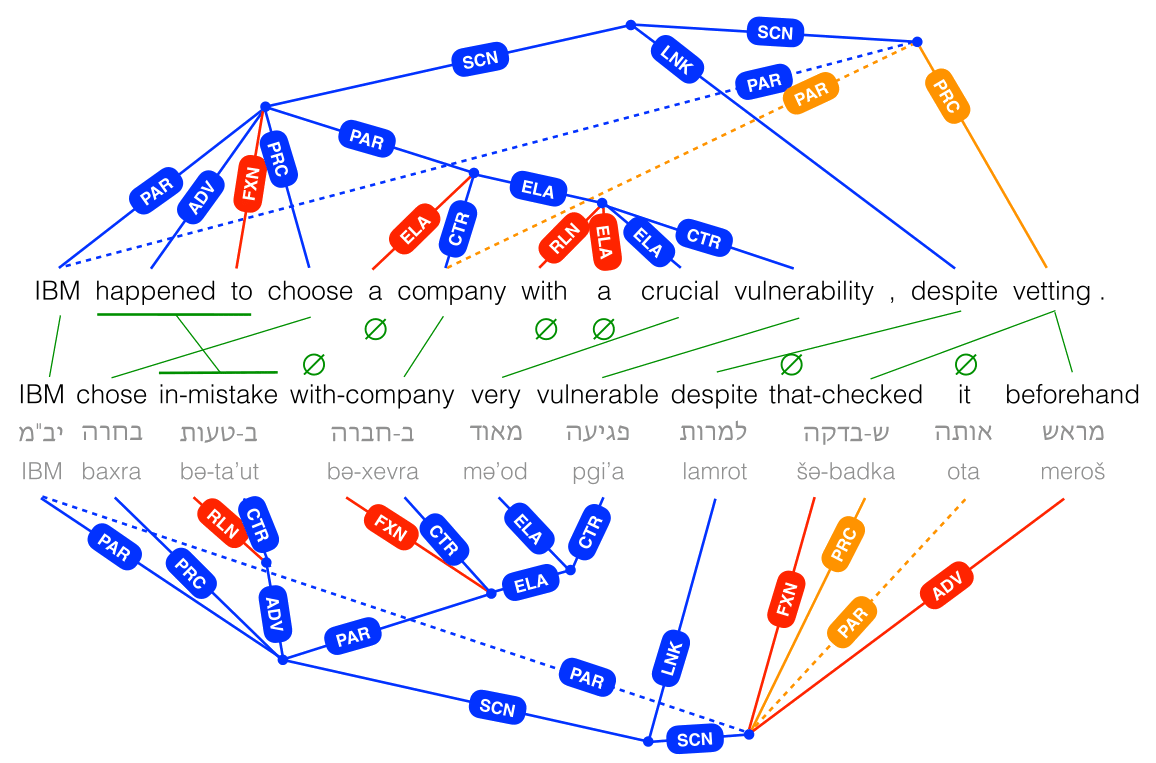
\includegraphics[width=\textwidth,height=\textheight,keepaspectratio]{crosslinguistic.png}
\end{adjustbox}
\\
\vspace{-1cm}
Hebrew
\end{frame}

\begin{frame}
\frametitle{Transition-Based UCCA Parsing}
Parse text $w_1 \ldots w_n$ to graph $G$ incrementally by applying transitions to the parser state:
stack, buffer and constructed graph.

\vfill
Initial state:
\begin{tikzpicture}[every node/.append style={font=\rmfamily}, circle]
	\draw[xstep=1cm,ystep=5mm,color=gray] (-0.01,0) grid (1,.5);
	\node[anchor=west,style={font=\sffamily}] at (-0.1,1.00)     {stack};
	\node[fill=black] at (0.5,0.25) {};
	\draw[xstep=1cm,ystep=5mm,color=gray] (3,0) grid (10,.5);
	\node[anchor=west,style={font=\sffamily}] at (8.9,1.00) {buffer};
	\node[anchor=west] at (3,0.25) {You};
	\node[anchor=west] at (4,0.25) {want};
	\node[anchor=west] at (5,0.25) {to};
	\node[anchor=west] at (6,0.25) {take};
	\node[anchor=west] at (7,0.25) {a};
	\node[anchor=west] at (8,0.25) {long};
	\node[anchor=west] at (9,0.25) {bath};
\end{tikzpicture}

\vfill
\parser{} \cite{hershcovich2017a} transitions:

\{\textsc{Shift, Reduce, Node$_X$, Left-Edge$_X$, Right-Edge$_X$,}\\
\hspace{5mm}\textsc{Left-Remote$_X$, Right-Remote$_X$, Swap, Finish}\}

\vfill
Support {\color{blue}non-terminal nodes}, {\color{orange}reentrancy} and {\color{red}discontinuity}.
\end{frame}

\begin{frame}
\frametitle{\parser{} Model}
Learns to greedily predict transition based on current state.

BiLSTM + MLP classifier \cite{kiperwasser2016simple}.

\vfill

Features:
words, POS, syntactic dependencies, existing edge labels \\
from the stack and buffer + parents, children, grandchildren;
ordinal features (height, number of parents and children)

\vspace{5mm}
\begin{tikzpicture}
	\draw[xstep=1cm,ystep=5mm,color=gray] (-0.01,0) grid (4,.5);
	\draw[xstep=1cm,ystep=5mm,color=gray] (5,0) grid (10,.5);
	\node[anchor=west] at (-0.1,1.00) {stack};
	\node[anchor=west] at (8.9,1.00) {buffer};
	\foreach \i in {0.5,8.5,9.5} {
		\node[fill=gray, circle] at (\i,0.25) {};
	}
	\foreach \i in {1.5,2.5,3.5,5.5,6.5,7.5} {
		\node[fill=black, circle] at (\i,0.25) {};
	}
\end{tikzpicture}
\end{frame}

\begin{frame}
\centering

\onslide<2>{
\fbox{
\begin{minipage}{.5\textwidth}
\begin{tikzpicture}[every node/.append style={font=\rmfamily}]
	\node[anchor=west,style={font=\sffamily}] at (-1.2,0.25){stack};
	\draw[xstep=1cm,ystep=5mm,color=gray] (-0.01,0) grid (4,.5);
	\node[fill=black, circle] at (0.5,0.25) {};
	\node[fill=blue, circle] at (2.5,0.25) {};
	\node[anchor=west] at (1,0.25) {You};
	\node[anchor=west] at (3,0.25) {take};
\end{tikzpicture}

\vspace{1cm}
\begin{tikzpicture}[every node/.append style={font=\rmfamily}]
	\node[anchor=west,style={font=\sffamily}] at (3.8,0.25){buffer};
	\draw[xstep=1cm,ystep=5mm,color=gray] (5,0) grid (9,.5);
	\node[fill=red, circle] at (5.5,0.25) {};
	\node[anchor=west] at (6,0.25) {a};
	\node[anchor=west] at (7,0.25) {long};
	\node[anchor=west] at (8,0.25) {bath};
\end{tikzpicture}
\end{minipage}
\begin{minipage}{.4\textwidth}
\scalebox{.8}{
\begin{tikzpicture}[level distance=1cm, sibling distance=1cm, ->,
    every node/.append style={font=\rmfamily}]
    \node[anchor=west,style={font=\sffamily}] at (5,0) {graph};
    \draw[color=gray] (1.2,.3) rectangle (4.9,-3.2);
    \node(ROOT)[fill=black, circle, visible on=<2->] at (3,0) {}
      child {node (You) {You} edge from parent node [left] {\scriptsize $A$}}
      child {node {want} edge from parent node [left] {\scriptsize $P$}}
      child {node (totakealongbath) [fill=blue, circle] {}
      {
        child {node {to} edge from parent node [left] {\scriptsize $F$}}
        child {node (takeabath) [fill=red, circle] {}
        {
          child {node {take} edge from parent node [right] {\scriptsize $C$}}
          child [opacity=0] {node {a} edge from parent node [right] {\scriptsize $F$}}
          child [opacity=0] {node (long) {long} edge from parent [draw=none]}
          child [opacity=0] {node {bath} edge from parent node [right] {\scriptsize $C$}}
        } edge from parent [draw=none]}
      } edge from parent [draw=none]}
      ;
\end{tikzpicture}
}
\end{minipage}
}
}

\scalebox{.7}{
\begin{tikzpicture}[->]
	\tiny
	\tikzstyle{main}=[circle, minimum size=7mm, draw=black!80, node distance=12mm]
	\foreach \i/\word in {1/{You},3/{want},5/{to},7/{take},9/{a},11/{long},13/{bath}} {
	    \node (x\i) at (\i,-1.3) {\Large\textrm\word};
	    \node[main, fill=white!100] (h\i) at (\i,0) {LSTM};
        \path (x\i) edge (h\i);
	    \node[main, fill=white!100] (i\i) at (\i.5,.8) {LSTM};
        \path (x\i) edge [bend right] (i\i);
	    \node[main, fill=white!100] (l\i) at (\i.5,2.3) {LSTM};
        \path (h\i) edge [bend left] (l\i);
        \path (i\i) edge (l\i);
	    \node[main, fill=white!100] (k\i) at (\i,3.1) {LSTM};
        \path (i\i) edge [bend left] (k\i);
        \path (h\i) edge [bend left] (k\i);
	}
	\foreach \current/\next in {1/3,3/5,5/7,7/9,9/11,11/13} {
        \path (h\current) edge (h\next);
        \path (i\next) edge (i\current);
        \path (l\current) edge (l\next);
        \path (k\next) edge (k\current);
	}
    \onslide<2>\node[main, fill=white!100] (mlp) at (7,4.6) {MLP};
	\onslide<2>\foreach \i in {5,7,9} {
        \path (l\i) edge (mlp);
        \path (k\i) edge (mlp);
    }
    \coordinate (state) at (10.5,6.5);
    \onslide<2>\path (state) edge [bend left] (mlp);
    \onslide<2>\node (transition) at (7,5.8) {\large\textsc{Node}$_C$};
    \onslide<2>\path (mlp) edge (transition);
\end{tikzpicture}
}
\end{frame}

\begin{frame}
\frametitle{Tackled Tasks}
We consider four schemes \cite{abend2013universal,banarescu2013abstract,oepen2016towards,nivre2016universal}:

	{
	\hfill
	  \color{Indigo}
	    \scalebox{.6}{
	    \begin{tikzpicture}[level distance=15mm, -{Latex[length=2mm]},
	        every node/.append style={font=\bf\ttfamily},
	        every circle node/.append style={fill=Indigo},
	      level 1/.style={sibling distance=29mm},
	      level 2/.style={sibling distance=18mm}]
	      \tikzstyle{word} = [font=\rmfamily,color=black]
	      \node[font=\bf\sffamily\Large] at (-4,0) {UCCA:};
      \node (ROOT) [circle] {}
        child {node (After) [word] {After} edge from parent node[above] {L}}
        child {node (graduation) [circle] {}
        {
          child {node [word] {graduation} edge from parent node[left] {P}}
        } edge from parent node[right] {H} }
        child {node [word] {,} edge from parent node[below] {U}}
        child {node (moved) [circle] {}
        {
          child {node (John) [word] {John} edge from parent node[left] {A}}
          child {node [word] {moved} edge from parent node[left] {P}}
          child {node [circle] {}
          {
            child {node [word] {to} edge from parent node[left] {R}}
            child {node [word] {Paris} edge from parent node[right] {C}}
          } edge from parent node[above] {A} }
        } edge from parent node[above] {H} }
        ;
      \draw[dashed,-{Latex[length=5mm]}] (graduation) to node [above] {A} (John);
	    \end{tikzpicture}
	    }
	}
	
	\vspace{-14mm}
	\hspace{-9mm}
	\scalebox{.9}{
	  \begin{tikzpicture}[-{Latex[length=2mm]}, color=DarkGreen, level distance=16mm,
	      every node/.append style={sloped,anchor=south,auto=false,font=\scriptsize\bf\ttfamily},
	      level 1/.style={sibling distance=24mm}]
	    \node[font=\bf\sffamily\small] at (-2.6,0) {AMR:};
    \node (ROOT) [ellipse] {move-01}
      child {node [ellipse] {after}
      {
            child {node (graduation) [ellipse] {graduate-01} edge from parent node {op1} }
      } edge from parent node {time} }
      child {node (John) [ellipse] {person}
      {
        child {node [ellipse] {name}
        {
            child {node [ellipse] {"John"} edge from parent node {op1} }
        } edge from parent node {name} }
      } edge from parent node {ARG0} }
      child {node [ellipse] {city}
      {
        child {node [ellipse] {name}
        {
            child {node [ellipse] {"Paris"} edge from parent node {op1} }
        } edge from parent node {name} }
      } edge from parent node {ARG2} }
      ;
      \draw (graduation) to node {ARG0} (John);
	  \end{tikzpicture}
	  }
	\vspace{-24mm}
	
	\begin{center}
	\hspace{2cm}{\color{NavyBlue}\bf\sffamily\scriptsize UD:}
	\end{center}
	
	\vspace{-9mm}
	
	\begin{flushright}
	\begin{minipage}{.5\textwidth}
	    \rmfamily
	    \scalebox{.7}{
	    \begin{dependency}[edge style={-{Latex[length=2mm]}, color=NavyBlue},
	        text only label, label style={above, color=NavyBlue, font=\bf\ttfamily}, font=\small]
	    \begin{deptext}[column sep=.8em,ampersand replacement=\^]
    After \^ graduation \^ , \^ John \^ moved \^ to \^ Paris \\
    \end{deptext}
        \depedge[edge unit distance=1em]{2}{1}{case}
        \depedge[edge unit distance=1em]{4}{3}{punct}
        \depedge[edge unit distance=1em, edge start x offset=-4mm]{5}{4}{nsubj}
        \depedge[edge unit distance=1em, edge end x offset=-3mm]{2}{5}{obl}
        \depedge[edge unit distance=1em]{7}{6}{case}
        \deproot[edge unit distance=1em]{5}{root}
        \depedge[edge unit distance=1.5em, edge start x offset=1mm]{5}{7}{obl}
    \end{dependency}
	}
	\end{minipage}
	
	\begin{minipage}{.06\textwidth}
	{\color{DarkRed}\bf\sffamily\scriptsize SDP:}
	\end{minipage}
	\begin{minipage}{.5\textwidth}
	    \rmfamily
	    \scalebox{.7}{
	    \begin{dependency}[edge style={-{Latex[length=2mm]}, color=DarkRed},
	        text only label, label style={above, color=DarkRed, font=\bf\ttfamily}, font=\small]
	    \begin{deptext}[column sep=.8em,ampersand replacement=\^]
    After \^ graduation \^ , \^ John \^ moved \^ to \^ Paris \\
    \end{deptext}
        \depedge[edge unit distance=1em]{1}{2}{ARG2}
        \depedge[edge unit distance=1em, edge start x offset=-4mm]{5}{4}{ARG1}
        \depedge[edge unit distance=1em, edge end x offset=-3mm]{1}{5}{ARG1}
        \deproot[edge unit distance=1.25em]{5}{top}
        \depedge[edge unit distance=2em, edge start x offset=1mm, edge end x offset=3mm]{5}{7}{ARG2}
        \depedge[edge unit distance=1em, edge end x offset=5mm]{6}{5}{ARG1}
        \depedge[edge unit distance=1em]{6}{7}{ARG2}
    \end{dependency}
	}
	\end{minipage}
	\end{flushright}
	
\end{frame}

\begin{frame}
\frametitle{Data}
	The amount of labeled data varies, e.g., in English:
	\begin{center}
	\pgfplotstableread[row sep=\\,col sep=&]{
		corpus & total \\
		\color{NavyBlue} \textbf{UD} & 17062 \\
		\color{DarkRed} \textbf{SDP} & 33964 \\
		\color{DarkGreen} \textbf{AMR} & 36521 \\
		\color{Indigo} \textbf{UCCA} & 5225 \\
	    }\english
	    \begin{tikzpicture}
	    \begin{axis}[
	    xbar stacked,
	    width=10cm,
	    height=39mm,
	    xmin=0,
	    xmax=60000,
	    xtick=\empty,
	    ytick=data,
	    yticklabels from table={\english}{corpus},
	    axis x line=none,
	    ]
	    \addplot [fill=Navy, point meta=explicit symbolic,
	    nodes near coords={\pgfmathprintnumber\pgfplotspointmeta~sentences},
	    nodes near coords align={anchor=west}] table [x=total,y expr=\coordindex,meta=total] {\english};
	    \end{axis}
	    \end{tikzpicture}
	\end{center}
	
	\pause
	\vfill
	
	Domains differ, too:
	\begin{center}
		\begin{tabular}{llll}
			\color{Indigo} \textbf{UCCA}  & \color{DarkGreen} \textbf{AMR}  & \color{DarkRed} \textbf{SDP}  & \color{NavyBlue} \textbf{UD}  \\
			Wikipedia & blogs & news & blogs \\ books & news && news \\ & emails && emails \\ & reviews && reviews \\ &&& Q\&A
		\end{tabular}
	\end{center}
\end{frame}

\begin{frame}
	\frametitle{Multitask Architecture}

    We treat UCCA parsing as the main task, \\ and AMR, SDP and UD as auxiliaries.	
	
	\begin{center}
		\fbox{\scalebox{.7}{
		\begin{minipage}{.5\textwidth}
		\begin{tikzpicture}[every node/.append style={font=\rmfamily}]
			\node[anchor=west,style={font=\sffamily}] at (-1.2,0.25){stack};
			\draw[xstep=1cm,ystep=5mm,color=gray] (-0.01,0) grid (4,.5);
			\node[fill=black, circle] at (0.5,0.25) {};
			\node[fill=blue, circle] at (2.5,0.25) {};
			\node[anchor=west] at (1,0.25) {You};
			\node[anchor=west] at (3,0.25) {take};
		\end{tikzpicture}
		
		\vspace{1cm}
		\begin{tikzpicture}[every node/.append style={font=\rmfamily}]
			\node[anchor=west,style={font=\sffamily}] at (3.8,0.25){buffer};
			\draw[xstep=1cm,ystep=5mm,color=gray] (5,0) grid (9,.5);
			\node[fill=red, circle] at (5.5,0.25) {};
			\node[anchor=west] at (6,0.25) {a};
			\node[anchor=west] at (7,0.25) {long};
			\node[anchor=west] at (8,0.25) {bath};
		\end{tikzpicture}
		\end{minipage}
		\begin{minipage}{.4\textwidth}
		\scalebox{.8}{
		\begin{tikzpicture}[level distance=1cm, sibling distance=1cm, ->,
		    every node/.append style={font=\rmfamily}]
		    \node[anchor=west,style={font=\sffamily}] at (5,0) {graph};
		    \draw[color=gray] (1.2,.3) rectangle (4.9,-3.2);
		    \node(ROOT)[fill=black, circle] at (3,0) {}
		      child {node (You) {You} edge from parent node [left] {\scriptsize $A$}}
		      child {node {want} edge from parent node [left] {\scriptsize $P$}}
		      child {node (totakealongbath) [fill=blue, circle] {}
		      {
		        child {node {to} edge from parent node [left] {\scriptsize $F$}}
		        child {node (takeabath) [fill=red, circle] {}
		        {
		          child {node {take} edge from parent node [right] {\scriptsize $C$}}
		          child [opacity=0] {node {a} edge from parent node [right] {\scriptsize $F$}}
		          child [opacity=0] {node (long) {long} edge from parent [draw=none]}
		          child [opacity=0] {node {bath} edge from parent node [right] {\scriptsize $C$}}
		        } edge from parent [draw=none]}
		      } edge from parent [draw=none]}
		      ;
		\end{tikzpicture}
		}
		\end{minipage}
		}}
		
		\scalebox{.3}{\Huge
		   \begin{tikzpicture}[-{Latex[length=3mm]},thick]
		   \tikzstyle{main}=[rounded rectangle, minimum size=23mm, draw=black!80, node distance=12mm]
		   \node[main] (specific) at (0,10) {Task-specific BiLSTM};
		   \node[main] (shared) at (22,10) {Shared BiLSTM};
		   \node (embeddings) at (10.5,4.5) {Shared embeddings};
		   \foreach \i/\word in {-4/{You},4/{want},17/{long},25/{bath}} {
		       \node (x\i) at (\i,3) {\word};
		       \node[main, minimum size=16mm] (e\i) at (\i,6) {};
		       \path (x\i) edge (e\i);
		       \path (e\i) edge (specific);
		       \path (e\i) edge (shared);
		   }
		    \node (x4) at (10.5,3) {\ldots};
		    \node[main] (mlp) at (10.5,12) {Task-specific MLP};
		    \path (specific) edge (mlp);
		    \path (shared) edge (mlp);
		    \coordinate (state) at (22,17);
		    \path (state) edge [bend left] (mlp);
		    \node (transition) at (10.5,16.4) {transition};
		    \path (mlp) edge node[right] {softmax} (transition);
		   \end{tikzpicture}}
   \end{center}
\end{frame}

\begin{frame}
\frametitle{Unified DAG Format}

We convert all representations into a format similar to UCCA and
supported by TUPA.

    \hspace{-5mm}
	\begin{minipage}{.4\textwidth}
	  \begin{center}
	  \begin{tikzpicture}[level distance=22mm, -{Latex[length=2mm]}, color=DarkGreen,
	      every node/.append style={sloped,anchor=south,auto=false,font=\scriptsize\bf\ttfamily},
	      level 1/.style={sibling distance=17mm},
	      level 2/.style={sibling distance=13mm},
	      level 3/.style={sibling distance=13mm}]
	    \tikzstyle{word} = [font=\rmfamily,color=black]
	    \node (ROOT) [word] {moved}
	      child {node [word] {After}
	      {
	            child {node (graduation) [word] {graduation} edge from parent node {op} }
	      } edge from parent node {time} }
	      child {node (John) [fill=DarkGreen,circle] {}
	      {
	        child {node [word] {John} edge from parent node {name} }
	      } edge from parent node {ARG0} }
	      child {node [fill=DarkGreen,circle] {}
	      {
	        child {node [word] {Paris} edge from parent node {name} }
	      } edge from parent node {ARG2} }
	      ;
	      \draw[dashed] (graduation) to node {ARG0} (John);
	  \end{tikzpicture}
	  \captionof{figure}{\color{DarkGreen} Converted AMR.}
	  \end{center}
	\end{minipage}
	\hfill
	\begin{minipage}{.5\textwidth}
	  \begin{center}
	  \scalebox{.7}{
	  \hspace{-13mm}
	  \begin{tikzpicture}[-{Latex[length=2mm]}, color=DarkRed,
	      every node/.append style={sloped,anchor=south,auto=false,font=\scriptsize\bf\ttfamily},
	      level 1/.style={sibling distance=28mm,level distance=13mm},
	      level 2/.style={sibling distance=16mm,level distance=15mm},
	      level 3/.style={level distance=18mm}]
	    \tikzstyle{word} = [font=\rmfamily,color=black]
	    \node (ROOT) [fill=DarkRed,circle] {}
	      child {node (after) [fill=DarkRed,circle] {}
	      {
	        child {node [draw=none] {}
	        {
	          child {node [word] (after_word) {After{\color{white}g}} edge from parent [draw=none]}
	        } edge from parent [draw=none] }
	        child {node [draw=none] {}
	        {
	          child {node [word] (graduation) {graduation ,} edge from parent [draw=none]}
	        } edge from parent [draw=none] }
	      } edge from parent node {root}}
	      child {node [draw=none] {}
	      {
	        child {node (moved) [fill=DarkRed,circle] {}
	        {
	          child {node [word] {\quad{\color{white}g} John} edge from parent node {ARG1}}
	          child {node [word] {moved{\color{white}g}} edge from parent node {head}}
	        } edge from parent [draw=none] }
	      } edge from parent [draw=none] }
	      child {node (to) [fill=DarkRed,circle] {}
	      {
	        child {node [draw=none] {}
	        {
	            child {node [word] (to_word) {to{\color{white}g}} edge from parent [draw=none]}
	          } edge from parent [draw=none] }
	          child {node [draw=none] {}
	        {
	          child {node [word] (Paris) {Paris{\color{white}g}} edge from parent [draw=none]}
	        } edge from parent [draw=none] }
	      } edge from parent node {root}}
	      ;
	      \draw (ROOT) to node {top} (moved);
	      \draw (after) to node {head} (after_word);
	      \draw (after) to node {ARG2} (graduation);
	      \draw[dashed] (after) to node {ARG1} (moved);
	      \draw[dashed] (to) to node {ARG1} (moved);
	      \draw (to) to node {head} (to_word);
	      \draw (moved) to node {ARG2} (Paris);
	      \draw[dashed] (to) to node {ARG2} (Paris);
	  \end{tikzpicture}}
	  \captionof{figure}{\color{DarkRed} Converted SDP.}
	  \vfill
	  \scalebox{.7}{
	  \hspace{-13mm}
	  \begin{tikzpicture}[-{Latex[length=2mm]}, color=DarkBlue,
	      every node/.append style={sloped,anchor=south,auto=false,font=\scriptsize\bf\ttfamily},
	      level 1/.style={sibling distance=16mm,level distance=13mm},
	      level 2/.style={sibling distance=14mm,level distance=15mm}]
	    \tikzstyle{word} = [font=\rmfamily,color=black]
	    \node (ROOT) [fill=DarkBlue,circle] {}
	      child {node (after) [fill=DarkBlue,circle] {}
	      {
	        child {node [word] {After{\color{white}g}\quad\quad} edge from parent node {case}}
	        child {node [word] {\quad graduation\quad\quad} edge from parent node {head}}
	      } edge from parent node {obl}}
	      child {node {}
	      {
	        child {node [word] (comma) {\quad,{\color{white}g}} edge from parent [draw=none]}
	      } edge from parent [draw=none]}
	      child {node {}
	      {
	        child {node [word] (John) {John{\color{white}g}} edge from parent [draw=none]}
	      } edge from parent [draw=none]}
	      child {node {}
	      {
	        child {node [word] (moved) {moved{\color{white}g}} edge from parent [draw=none]}
	      } edge from parent [draw=none]}
	      child {node (to) [fill=DarkBlue,circle] {}
	      {
	          child {node [word] {to{\color{white}g}} edge from parent node {case}}
	          child {node [word] {Paris{\color{white}g}} edge from parent node {head}}
	      } edge from parent node {obl}}
	      ;
	      \draw (ROOT) to node {punct} (comma);
	      \draw (ROOT) to node {nsubj} (John);
	      \draw (ROOT) to node {head} (moved);
	  \end{tikzpicture}}
	  \captionof{figure}{\color{DarkBlue} Converted UD.}
	  \end{center}
	\end{minipage}

\end{frame}

\begin{frame}
\frametitle{UCCA Evaluation}
Comparing graphs over the same sequence of tokens,
\begin{itemize}
\item Match edges by their terminal yield and label.
\item Calculate \textbf{labeled precision, recall and F1} scores.
\item Separate primary (---) and remote (- - -) edges.
\end{itemize}
\vfill
\begin{adjustbox}{frame,scale=.75,center}
	\begin{tikzpicture}[level distance=15mm, sibling distance=15mm, ->,
	    every circle node/.append style={fill=black}]
	  \tikzstyle{word} = [font=\rmfamily,color=black]
	  \node at (-1,.7) {gold};
	  \node (ROOT) at (0,0) [circle] {}
	    child {node (After) [word] {After} edge from parent node[left] {$L$}}
	    child {node (graduation) [circle] {}
	    {
	      child {node [word] {graduation} edge from parent node[left] {$P$}}
	    } edge from parent node[left] {$H$} }
	    child {node [word] {,} edge from parent node[right] {$U$}}
	    child {node (moved) [circle] {}
	    {
	      child {node (Joe) [word] {Joe} edge from parent node[left] {$A$}}
	      child {node [word] {moved} edge from parent node[left] {$P$}}
	      child {node [circle] {}
	      {
	        child {node [word] {to} edge from parent node[left] {$R$}}
	        child {node [word] {Paris} edge from parent node[right] {$C$}}
	      } edge from parent node[right] {$A$} }
	    } edge from parent node[right] {$H$} }
	    ;
	  \draw[dashed,->] (graduation) to node [auto] {$A$} (Joe);
	  \node at (6,.7) {predicted};
	  \node (ROOT_) at (7,0) [circle] {}
	    child {node (After_) [word] {After} edge from parent node[left] {$L$}}
	    child {node (graduation_) [circle] {}
	    {
	      child[red] {node [word] {graduation} edge from parent node[left] {$S$}}
	    } edge from parent node[left] {$H$} }
	    child {node [word] {,} edge from parent node[right] {$U$}}
	    child {node (moved) [circle,xshift=3mm,yshift=-7mm] {}
	    {
	      child {node (Joe_) [word] {Joe} edge from parent node[left] {$A$}}
	      child {node [word] {moved} edge from parent node[left] {$P$}}
	      child[red] {node [word] {to} edge from parent node[left] {$F$}}
	      child[red] {node (Paris_) [word] {Paris} edge from parent node[right] {$A$}}
	    } edge from parent node[right] {$H$} }
	    ;
	  \draw[bend left,dashed,->] (graduation_) to node [auto] {$A$} (Joe_);
	  \draw[bend left,dashed,->,red] (graduation_) to node [auto] {$A$} (Paris_);
	\end{tikzpicture}
\end{adjustbox}
\vfill
\begin{adjustbox}{scale=.75,center}
	Primary:
	\begin{tabular}{ccc}
		\textbf{LP} & \textbf{LR} & \textbf{LF} \\ \hline
		$\frac69=67\%$ & $\frac6{10}=60\%$ & 64\%
	\end{tabular}
	\hspace{1cm}
	Remote:
	\begin{tabular}{ccc}
		\textbf{LP} & \textbf{LR} & \textbf{LF} \\ \hline
		$\frac12=50\%$ & $\frac11=100\%$ & 67\%
	\end{tabular}
\end{adjustbox}
\end{frame}

\begin{frame}
\frametitle{In-Domain Results}
Training on English Wikipedia UCCA (+ auxiliary) \\ Testing on English Wikipedia UCCA
\begin{center}
	\begin{tabular}{l|lll|lll}
	& \multicolumn{3}{c|}{Primary edges} & \multicolumn{3}{c}{Remote edges} \\
	& \textbf{LP} & \textbf{LR} & \textbf{LF}
	& \textbf{LP} & \textbf{LR} & \textbf{LF} \\
	\hline
	Single-task
	& 74.4 & 72.9 & 73.6 & 53 & 50 & 51.5 \\
	\cline{1-1}
	AMR
	& 74.7 & 72.8 & 73.7 & 48.7$\star$ & 51.1 & 49.9 \\
	DM
	& 75.7$\star$ & 73.9$\star$ & 74.8$\star$ & 54.9 & 53 & \textbf{53.9} \\
	UD$^{++}$
	& 75$\star$ & 73.2 & 74.1$\star$ & 49 & 52.7 & 50.8 \\
	AMR + DM
	& 75.6$\star$ & 73.9$\star$ & 74.7$\star$ & 49.9 & 53 & 51.4 \\
	AMR + UD$^{++}$
	& 74.9 & 72.7 & 73.8 & 47.1 & 50 & 48.5 \\
	DM + UD$^{++}$
	& 75.9$\star$ & 73.9$\star$ & \textbf{74.9}$\star$ & 48 & 54.8 & 51.2 \\
	All
	& 75.6$\star$ & 73.1 & 74.4$\star$ & 50.9 & 53.2 & 52
	\end{tabular}
\end{center}
\end{frame}

\begin{frame}
\frametitle{Out-of-Domain Results}
Training on English Wikipedia UCCA (+ auxiliary) \\ Testing on English \textbf{20K Leagues} UCCA
\begin{center}
	\begin{tabular}{l|lll|lll}
	& \multicolumn{3}{c|}{Primary edges} & \multicolumn{3}{c}{Remote edges} \\
	& \textbf{LP} & \textbf{LR} & \textbf{LF}
	& \textbf{LP} & \textbf{LR} & \textbf{LF} \\
	\hline
	Single-task
	& 69 & 69 & 69 & 41.2 & 19.8 & 26.7 \\
	\cline{1-1}
	AMR
	& 69.5 & 69.5 & 69.5 & 42.9 & 20.2 & 27.5 \\
	DM
	& 70.7$\star$ & 70.7$\star$ & 70.7$\star$ & 42.7 & 18.6 & 25.9 \\
	UD$^{++}$
	& 69.6 & 69.8$\star$ & 69.7 & 41.4 & 22 & 28.7 \\
	AMR + DM
	& 70.7$\star$ & 70.2$\star$ & 70.5$\star$ & 45.8 & 19.4 & 27.3 \\
	AMR + UD$^{++}$
	& 70.2$\star$ & 69.9$\star$ & 70$\star$ & 45.1 & 21.8 & 29.4 \\
	DM + UD$^{++}$
	& 70.8$\star$ & 70.3$\star$ & 70.6$\star$ & 41.6 & 21.6 & 28.4 \\
	All
	& 71.2$\star$ & 70.9$\star$ & \textbf{71}$\star$ & 45.1 & 22 & \textbf{29.6}
	\end{tabular}
\end{center}
\end{frame}

\begin{frame}
\frametitle{French and German Results}
Training on French/German 20K Leagues UCCA (+ auxiliary) \\ Testing on French/German 20K Leagues UCCA
\begin{center}
	\begin{tabular}{l|lll|lll}
	& \multicolumn{3}{c|}{Primary edges} & \multicolumn{3}{c}{Remote edges} \\
	& \textbf{LP} & \textbf{LR} & \textbf{LF}
	& \textbf{LP} & \textbf{LR} & \textbf{LF} \\
	\hline
	\multicolumn{4}{l|}{\bf French (in-domain)} & \\
	Single-task & 68.2 & 67 & 67.6 & 26 & \enskip 9.4 & 13.9 \\
	UD & 70.3 & 70$\star$ & \textbf{70.1}$\star$ & 43.8 & 13.2 & 20.3 \\
	\hline\\
	\multicolumn{4}{l|}{\bf German (in-domain)} & \\
	Single-task & 73.3 & 71.7 & 72.5 & 57.1 & 17.7 & 27.1 \\
	UD & 73.7$\star$ & 72.6$\star$ & \textbf{73.2}$\star$ & 61.8 & 24.9$\star$ & \textbf{35.5}$\star$
	\end{tabular}
\end{center}
\end{frame}



\begin{frame}
\frametitle{Conclusion}
\begin{itemize}
 \item Multitask learning improves UCCA parsing.
 \item \parser{} supports UCCA, AMR, SDP and UD with a uniform transition system and DAG format.
\end{itemize}

Future work:
\begin{itemize}
 \item Examination of the factors contributing to MTL success.
 \item AMR, SDP and UD parsing as main tasks. Preliminary experiments show promising results.
\end{itemize}

\end{frame}



\begin{frame}[allowframebreaks]
\frametitle{References}
\bibliographystyle{apalike}
\tiny\bibliography{references}
\end{frame}

\end{document}
